\documentclass[12pt,a4paper]{instrumentacao}

\usepackage{listings}
\usepackage{etoolbox}

\newtoggle{attachments}
\togglefalse{attachments}

\graphicspath{
	{../Resources/Images/}
	{../Resources/Mathematica/images/}
	{../Resources/MATLAB/images/}
}

\title{Central meteorológica: Dispositivo para medição de precipitação, de temperatura e de velocidade do vento}
\author{Rogiel Sulzbach \and Rodrigo de Castro Silveira \and Yi Chen Wu}
\startdate{28 de março de 2016}
\finishdate{18 de abril de 2016}
\emails{
	\emailaddress{R.J.S.}{rogiel@rogiel.com},
	\emailaddress{R.C.S.}{csilveira.rodrigo@gmail.com} e
	\emailaddress{Y.C.}{yichenpoa@gmail.com}
}
\resume{}
\abstract{}
\keywords{}
\institute{Universidade Federal do Rio Grande do Sul, Departamento de Engenharia Elétrica, Curso de Engenharia Elétrica, Instrumentação A, Profs. Dr. Alexandre Balbinot e Dra. Léia Bagesteiro}

\headertext{Anteprojeto}

\begin{document}
\maketitle

\todo{mudar a letra para times new roman.......}

\chapter{Introdução}
De acordo com o livro-texto da disciplina \textit{ENG04457 - Instrumentação A} \cite{livro-texto}, em seu prefácio, expõe que "hoje o mundo não escreve: digita. Internet, iPod, celulares, pen-drives... Toda essa revolução na sociedade criou novas habilitações dentro das engenharias, como, por exemplo, as engenharias de computação, de software e de tecnologia da informação. O analógico aparentemente tornou-se obsoleto, tirando a atenção de disciplinas relacionadas, como instrumentação, sensores e transdutores -- um equívoco ocorrido em função da compreensão superficial do que está por trás desta revolução tecnológica que estamos vivendo. Porém, o som, a imagem e diversos outros fenômenos que nos cercam são entes analógicos. Antes de virar bytes, o mundo é captado analogicamente". É com base nesta necessidade do domínio da captação do mundo analógico que a disciplina corretamente propõe a elaboração, planejamento e montagem de um projeto experimental utilizando os conceitos vistos em sala de aula.

O grupo, orientado por algumas indicações do professor da disciplina, optou pela elaboração do projeto de uma \textit{Central Meteorológica} capaz de executar medições de precipitação (chuva), de temperatura e de velocidade do vento. De acordo com a enciclopédia eletrônica livre \textit{Wikipedia}\cite{estacao}, "uma estação meteorológica é um local onde são recolhidos dados para análise do tempo meteorológico. Encontram-se equipadas com instrumentos (ou sensores eletrônicos) de medição e registro das variáveis meteorológicas/climáticas. Os seus dados são utilizados para a previsão do tempo e para a caracterização do clima, pelo que também podem ser designadas por estações climatológicas".

O projeto desenvolvido pelo grupo fará a captação e tratamento dos dados de temperatura, velocidade do vento e volume de precipitação. Assim, serão projetados os seguintes instrumentos:

\begin{itemize}
	\item \textbf{Termômetro}: para medir a temperatura;
	\item \textbf{Anemômetro}: para medir a velocidade do vento;
	\item \textbf{Pluviômetro}: para medir a precipitação pluviométrica.
\end{itemize}

\chapter{Metodologia Experimental}
A seguir serão apresentadas as especificações de cada um dos instrumentos a serem projetados e implementados para a montagem da Central Meteorológica, objeto do projeto final da disciplina.

\section{Termômetro}


\section{Anemômetro}
O anemômetro é um instrumento que mede a velocidade do vento horizontal. Os anemômetros de copo são o tipo padrão de anemômetro, pois são robustos e resistentes aos ventos oblíquos causados por mastros e travessas, e este tipo será utilizado no projeto em questão, a exemplo da Figura \ref{fig:anemometro}

\begin{figure}[h]
	\centering
		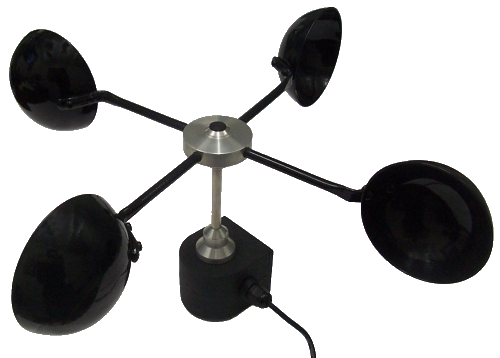
\includegraphics{Figuras/anemometro.png}
	\caption{Exemplo de anemômetro de copo}
	Fonte: \url{https://www.google.com.br/url?sa=i&rct=j&q=&esrc=s&source=images&cd=&cad=rja&uact=8&ved=&url=http%3A%2F%2Fwww.seinstrumentos.com.br%2Fanemometro.html&psig=AFQjCNGjijn5ng5hpmUAcBq4F_TVvceWUw&ust=1461032511805601}
	\label{fig:anemometro}
\end{figure}

Como forma de medir a velocidade de rotação do anemômetro, será utilizado um sensor de efeito \textit{Hall} associado com um ímã. Assim, toda vez que o ímã passar pelo sensor de efeito \textit{Hall}, este deixa passar corrente, podendo assim ser contabilizado o número de voltas em um determinado período de análise.


\section{Pluviômetro}
O pluviômetro é um dispositivo de meteorologia usado para recolher e medir, em milímetros, a quantidade de líquidos ou sólidos (chuva, neve, granizo) precipitados durante um determinado tempo e local. Tal aparelho é muito usado nas estações meteorológicas. Como o equipamento mensura a quantidade de chuva que precipita, é elementar para estudos meteorológicos e hidrológicos em conjunto com o sensor de temperatura. Um dos princípios de funcionamento composto é feito por um sensor de precipitação tipo báscula, um equipamento que mensura a massa de um corpo, pois o índice pluviométrico em milímetros indica o volume em litros de água que caíram em um metro quadrado de área, assim uma chuva de 20 mm corresponderá à precipitação de 20 litros de água por metro quadrado, logicamente sempre na horizontal. Como quaisquer equipamentos automáticos, um software de coleta e tratamento de dados é utilizado para relatórios temporais e análises das características da chuva. Como a maneira de medir a quantidade de chuva é muito ampla, cabe-se os membros do grupo investigar o melhor tipo de sensor e metodologia de medição apropriados para obter boas medidas. 

Segundo a Wikipedia \cite{pluviometro}, "o pluviômetro é um aparelho de meteorologia usado para recolher e medir, em milímetros lineares, a quantidade de líquidos ou sólidos (chuva, neve, granizo) precipitados durante um determinado tempo e local". O parâmetro determinado por esse instrumento chama-se \textit{índice pluviométrico}, que é o somatório da precipitação num determinado local durante um período de tempo estabelecido, medido em milímetros [$mm$].

A estrutura física do pluviômetro consiste em um sistema de captação de chuva, com uma área determinada, e um reservatório para coleta do material captado. Nesse reservatório há um sensor que possibilita medir a diferença do nível de fluído armazenado.

Optou-se, dentre os vários métodos de medição de nível, a medição por ultrassom. O princípio de funcionamento desse método é medir o tempo de eco de um sinal enviado por um transdutor piezoelétrico. O transdutor que transmite o sinal também pode fazer a leitura (ou podem ser módulos separados emissor-receptor). Quando esse transdutor atua como transmissor, é excitado com um sinal elétrico gerando uma onda mecânica. Quando atua como receptor, o transdutor recebe um sinal mecânico e converte-o em sinal elétrico \cite{livro-texto}. O tempo entre o sinal enviado e o sinal de eco corresponde ao dobro da distância entre o medidor e a superfície cujo nível está sendo medido, conforme exemplifica a equação \ref{eq:dist_ultrassom}.

\begin{equation}
	d=(vt)/2
	\label{eq:dist_ultrassom}
\end{equation}
>>>>>>> origin/master



\chapter{Cronograma de Execução}

Na Tabela \ref{tab:cronograma} é apresentado o cronograma de execução do projeto, tendo como premissa que "um bom projeto experimental obrigatoriamente deve ter um excelente planejamento experimental" \cite{livro-texto}.

\begin{table}[H]
\centering
\caption{Cronograma de execução do projeto}
\label{tab:cronograma}
\begin{tabular}{|c|l|}
\hline
\textit{\textbf{Prazo}} & \multicolumn{1}{c|}{\textit{\textbf{Atividades}}}               \\ \hline
18/abr                  & Entrega da Proposta do Projeto Final                            \\ \hline
20/abr                  & Compra de sensores e componentes                                \\ \hline
27/abr                  & Construção mecânica do anemômetro e do pluviômetro              \\ \hline
04/mai                  & Levantamento das curvas dos sensores                            \\ \hline
11/mai                  & Elaboração da interface homem-máquina no LABView                \\ \hline
18/mai                  & Design e montagem de placa de circuito impresso                 \\ \hline
25/mai                  & Testes e análise de incertezas dos sensores                     \\ \hline
01/jun                  & Finalização do Anteprojeto                                      \\ \hline
06/jun                  & Apresentação do Anteprojeto                                     \\ \hline
08/jun                  & Ajuste da interface gráfica                                     \\ \hline
15/jun                  & Ajustes, testes finais e finalização da documentação do projeto \\ \hline
22/jun                  & Ajustes, testes finais e finalização da documentação do projeto \\ \hline
27/jun                  & Apresentação do Projeto Final                                   \\ \hline
\end{tabular}
\end{table}


\chapter{Conclusões}

\iftoggle{attachments}{
	\chapter*{Anexos}
	\section{Mathematica}

	\section{LabVIEW}

	\section{MATLAB}
}

\begin{thebibliography}{9}
\bibitem{mathematica-numerial-precision} \url{https://reference.wolfram.com/language/tutorial/NumericalPrecision.html}, acessado em 16 de março de 2016

\bibitem{livro-texto}  Balbinot, A.; Brusamarello, V. J., Instrumentação e Fundamentos de Medida - Vol.1 - 2ª Ed. Rio de Janeiro: LTC, 2014.

\bibitem{estacao} \url{https://pt.wikipedia.org/wiki/Esta%C3%A7%C3%A3o_meteorol%C3%B3gica}, acessado em 16/04/2016.

\bibitem{pluviometro} \url{https://pt.wikipedia.org/wiki/Pluvi%C3%B4metro}, acessado em 16/04/2016.
\bibitem{pluviometro-1} \url{http://www.agsolve.com.br/dicas-e-solucoes/como-funciona-o-pluviometro}, acessado em 16/04/2016.



%\bibitem{ref1} Sobrenome, A.B.; Sobrenome, C.D. Title of the cited article. Journal Title 2007, 6, 100-110. 
%\bibitem{ref2} Balbinot, A.; Brusamarello, V.J.. Title of the cited article. Journal Title 2007, 6, 100-110. 
%\bibitem{ref3} Author, A.; Author, B. Title of the chapter. In Book Title, 2nd ed.; Editor, A., Editor, B., Eds.; Publisher: Publisher Location, Country, 2007; Volume 3, pp. 154-196.
%\bibitem{ref4} Author, A.; Author, B. Book Title, 3rd ed.; Publisher: Publisher Location, Country, 2008; 
%pp. 154-196.

\end{thebibliography}

\end{document}
